\documentclass[12pt, titlepage]{article}

\usepackage{fullpage}
\usepackage[round]{natbib}
\usepackage{booktabs}
\usepackage{tabularx}
\usepackage{graphicx}
\usepackage{float}
\usepackage{longtable}
\usepackage{tikz}
\usetikzlibrary{positioning,arrows.meta}
\usepackage{hyperref}
\hypersetup{
    colorlinks,
    citecolor=blue,
    filecolor=black,
    linkcolor=red,
    urlcolor=blue
}

\input{../../Comments.text}
\commentsfalse
\input{../../Common.text}

\newcounter{acnum}
\newcommand{\actheacnum}{AC\theacnum}
\newcommand{\acref}[1]{AC\ref{#1}}

\newcounter{ucnum}
\newcommand{\uctheucnum}{UC\theucnum}
\newcommand{\uref}[1]{UC\ref{#1}}

\newcounter{mnum}
\newcommand{\mthemnum}{M\themnum}
\newcommand{\mref}[1]{M\ref{#1}}

\begin{document}

\title{Module Guide for \progname{}}
\author{\authname}
\date{\today}

\maketitle

\pagenumbering{roman}

\section{Revision History}

\begin{tabularx}{\textwidth}{p{3cm}p{2cm}X}
\toprule {\bf Date} & {\bf Version} & {\bf Notes}\\
\midrule
Nov 13, 2026 & 0.1 & Tyler Yue: Initial Rev~-1 draft including anticipated and
unlikely changes, module hierarchy, secrets/services, requirements connection,
traceability matrices, and uses hierarchy.\\
Nov 13, 2026 & 0.2 & Tyler Yue: Edited the Rev~-1 to ensure it is aligned with the rubric and the Module Guide.\\
\bottomrule
\end{tabularx}

\newpage

\section{Reference Material}

This section records information for easy reference.

\subsection{Abbreviations and Acronyms}

\renewcommand{\arraystretch}{1.2}
\begin{tabular}{l l}
  \toprule
  \textbf{symbol} & \textbf{description}\\
  \midrule
  AC & Anticipated Change\\
  AO & Abstract Object\\
  DAG & Directed Acyclic Graph\\
  FR & Functional Requirement (SRS)\\
  HA & Hazard Analysis\\
  IDE & Integrated Development Environment\\
  JML & Java Modeling Language\\
  LLM & Large Language Model\\
  M & Module\\
  MG & Module Guide\\
  MIS & Module Interface Specification\\
  NFR & Nonfunctional Requirement (SRS)\\
  OS & Operating System\\
  SRS & Software Requirements Specification\\
  SR & Safety/Security Requirement (Hazard Analysis)\\
  UC & Unlikely Change\\
  VnV & Verification and Validation\\
  \bottomrule
\end{tabular}\\

\subsection{Related Documents}

\begin{itemize}
  \item Software Requirements Specification (Volere):
  \texttt{docs/SRS-Volere/SRS.tex}
  \item Hazard Analysis: \texttt{docs/HazardAnalysis/HazardAnalysis.tex}
  \item Verification and Validation Plan: \texttt{docs/VnVPlan/VnVPlan.tex}
  \item Module Interface Specification:
  \texttt{docs/Design/SoftDetailedDes/MIS.tex}
  \item Development Plan: \texttt{docs/DevelopmentPlan/DevelopmentPlan.tex}
\end{itemize}

\newpage

\tableofcontents

\listoftables

\listoffigures

\newpage

\pagenumbering{arabic}

\section{Introduction}

Decomposing a system into modules is a commonly accepted approach to developing
software. A module is a work assignment for a programmer or programming
team~\citep{ParnasEtAl1984}. We advocate a decomposition based on the principle
of information hiding~\citep{Parnas1972a}. This principle supports design for
change, because the ``secrets'' that each module hides represent likely future
changes.

Our design follows the rules laid out by \citet{ParnasEtAl1984}, as follows:
\begin{itemize}
\item System details that are likely to change independently should be the
  secrets of separate modules.
\item Each data structure is implemented in only one module.
\item Any other program that requires information stored in a module's data
  structures must obtain it by calling access programs belonging to that module.
\end{itemize}

After completing the Software Requirements Specification (SRS), the Module Guide
(MG) is developed~\citep{ParnasEtAl1984}. The MG specifies the modular structure
of the system and is intended to allow both designers and maintainers to easily
identify the parts of the software. The potential readers of this document are
as follows:

\begin{itemize}
\item New project members: a guide to the overall structure and the location of
  relevant modules.
\item Maintainers: the hierarchy supports understanding when changes are made;
  maintainers should update this document after structural changes.
\item Designers: a check for consistency, feasibility, and flexibility of the
  decomposition.
\end{itemize}

\progname{} is a VS~Code extension that captures engineering intent from a
developer request, requires human approval of proposed artifacts, stores an
intent model with rationale and traceability, and verifies AI-generated changes
against that model. This Rev~-1 Module Guide records the architecture
(secrets, services, uses relation, and requirement traceability). Detailed
interface syntax appears in the companion MIS. Full MIS semantics and design
reflection are deferred to Revision~0, consistent with the course Des.\ Doc.\
Rev~-1 requirements.

The rest of the document is organized as follows. Section~\ref{SecChange} lists
anticipated and unlikely changes. Section~\ref{SecMH} summarizes the module
hierarchy. Section~\ref{SecConnection} records design decisions that connect
requirements to the architecture. Section~\ref{SecMD} describes each module's
secrets and services. Section~\ref{SecTM} gives traceability matrices.
Section~\ref{SecUse} describes the uses hierarchy.

\section{Anticipated and Unlikely Changes} \label{SecChange}

\subsection{Anticipated Changes} \label{SecAchange}

Anticipated changes are the source of the information hidden inside modules.
Ideally, changing one anticipated change requires changing only the module that
hides the associated decision.

\begin{description}
\item[\refstepcounter{acnum} \actheacnum \label{acHostIDE}:] The host IDE and
  its extension API (currently VS~Code; Cursor and other hosts may be added).
\item[\refstepcounter{acnum} \actheacnum \label{acInputForms}:] The set of
  supported engineering-artifact input forms beyond natural language (for
  example UML or Petri-net submissions).
\item[\refstepcounter{acnum} \actheacnum \label{acElicitation}:] The elicitation
  strategy and orchestration used to refine a request into requirements and
  constraints (prompts, graph structure, clarification policy).
\item[\refstepcounter{acnum} \actheacnum \label{acSchema}:] The schema and file
  layout of the versioned intent model in the workspace.
\item[\refstepcounter{acnum} \actheacnum \label{acAssistant}:] The integration
  mechanism used to instruct and receive proposals from an AI coding assistant
  (the concrete protocol and message shapes are hidden by the adapter module).
\item[\refstepcounter{acnum} \actheacnum \label{acContracts}:] The executable
  contract language and compilation strategy used for approved requirements
  (the concrete notation is a secret of the Contract Compiler).
\item[\refstepcounter{acnum} \actheacnum \label{acVerifier}:] The external
  checker used to verify generated implementations against contracts (the tool
  choice and invocation details are secrets of the Contract Verifier).
\item[\refstepcounter{acnum} \actheacnum \label{acReviewUX}:] The presentation
  and interaction design of the review panel inside the host IDE.
\item[\refstepcounter{acnum} \actheacnum \label{acTrace}:] The representation and
  justification format of traceability links between intent elements, code, and
  tests.
\item[\refstepcounter{acnum} \actheacnum \label{acPrivacy}:] The policy for what
  project content may leave the machine for LLM or tracing services.
\item[\refstepcounter{acnum} \actheacnum \label{acLogging}:] The diagnostic log
  format and retention policy for failures and significant interactions.
\end{description}

\subsection{Unlikely Changes} \label{SecUchange}

The following decisions are fixed for this architecture. Changing them would
force widespread redesign.

\begin{description}
\item[\refstepcounter{ucnum} \uctheucnum \label{ucHumanGate}:] A human developer
  must approve, edit, or reject proposed engineering artifacts before they may
  guide code generation (human-in-the-loop gate).
\item[\refstepcounter{ucnum} \uctheucnum \label{ucLocalWorkspace}:] The product
  operates on a single local developer workspace; multi-user concurrent editing
  of one intent model is out of scope for the capstone.
\item[\refstepcounter{ucnum} \uctheucnum \label{ucIntentSource}:] Approved intent
  is the source of truth for what the AI coding assistant may implement; chat
  history alone is not authoritative.
\item[\refstepcounter{ucnum} \uctheucnum \label{ucGitVersioning}:] The intent
  model is versioned with the project using Git-compatible storage in the
  workspace.
\item[\refstepcounter{ucnum} \uctheucnum \label{ucExtensionForm}:] The primary
  user interaction surface is an IDE extension embedded in the host editor,
  not a standalone desktop application.
\end{description}

\section{Module Hierarchy} \label{SecMH}

This section provides an overview of the module design. Each leaf module is a
work assignment for a programmer in the sense of \citet{ParnasEtAl1984}: one
cohesive secret, a small set of services, and a clear uses relationship to peer
modules. Modules are summarized in a hierarchy decomposed by secrets in
Table~\ref{TblMH}. The leaf modules in the hierarchy are the modules that will
be implemented.

\begin{description}
\item [\refstepcounter{mnum} \mthemnum \label{mHH}:] Hardware-Hiding Module
\item [\refstepcounter{mnum} \mthemnum \label{mHost}:] Host IDE Interface Module
\item [\refstepcounter{mnum} \mthemnum \label{mBH}:] Behaviour-Hiding Module
\item [\refstepcounter{mnum} \mthemnum \label{mControl}:] Workflow Controller Module
\item [\refstepcounter{mnum} \mthemnum \label{mCapture}:] Intent Capture Module
\item [\refstepcounter{mnum} \mthemnum \label{mReview}:] Review Panel Module
\item [\refstepcounter{mnum} \mthemnum \label{mGate}:] Approval Gate Module
\item [\refstepcounter{mnum} \mthemnum \label{mReport}:] Verification Report Module
\item [\refstepcounter{mnum} \mthemnum \label{mSD}:] Software Decision Module
\item [\refstepcounter{mnum} \mthemnum \label{mStore}:] Intent Model Store Module
\item [\refstepcounter{mnum} \mthemnum \label{mTrace}:] Traceability Manager Module
\item [\refstepcounter{mnum} \mthemnum \label{mElicit}:] Elicitation Engine Module
\item [\refstepcounter{mnum} \mthemnum \label{mCompile}:] Contract Compiler Module
\item [\refstepcounter{mnum} \mthemnum \label{mVerify}:] Contract Verifier Module
\item [\refstepcounter{mnum} \mthemnum \label{mAssist}:] Coding Assistant Adapter Module
\item [\refstepcounter{mnum} \mthemnum \label{mLog}:] Diagnostic Log Module
\end{description}

\begin{table}[H]
\centering
\begin{tabular}{p{0.32\textwidth} p{0.58\textwidth}}
\toprule
\textbf{Level 1} & \textbf{Level 2}\\
\midrule
Hardware-Hiding Module & Host IDE Interface Module\\
\midrule
Behaviour-Hiding Module & Workflow Controller Module\\
 & Intent Capture Module\\
 & Review Panel Module\\
 & Approval Gate Module\\
 & Verification Report Module\\
\midrule
Software Decision Module & Intent Model Store Module\\
 & Traceability Manager Module\\
 & Elicitation Engine Module\\
 & Contract Compiler Module\\
 & Contract Verifier Module\\
 & Coding Assistant Adapter Module\\
 & Diagnostic Log Module\\
\bottomrule
\end{tabular}
\caption{Module Hierarchy}
\label{TblMH}
\end{table}

\section{Connection Between Requirements and Design} \label{SecConnection}

The design satisfies the SRS and related Hazard Analysis safety requirements
through the following explicit decisions made between requirements and
architecture:

\begin{itemize}
  \item \textbf{Human approval before generation (FR7, FR8, SCR1, HA-SR6,
  HA-SR7).} The Approval Gate Module is the sole authority that records a
  developer decision and releases an instruction to the coding assistant. The
  assistant adapter never exposes approve/reject as assistant-callable tools.
  \item \textbf{Intent model as source of truth (FR9, FR11, HA-SR9).} Approved
  artifacts, rationale, and history live only in the Intent Model Store. Other
  modules obtain intent exclusively through that module's access programs.
  \item \textbf{Traceability as a first-class structure (FR9, FR11, EUR3,
  HA-SR10).} Links and justifications are owned by the Traceability Manager so
  that missing or broken links can be reported independently of storage format.
  \item \textbf{Executable contracts for constrained generation (FR12,
  HA-SR11).} Approved requirements are compiled into checkable contracts by the
  Contract Compiler; the Contract Verifier reports pass/fail evidence without
  treating infrastructure failure as success.
  \item \textbf{Host isolation (AR1, ACCR1, MR2).} All IDE-specific presentation
  and workspace I/O go through the Host IDE Interface so that host migration
  does not rewrite behavioural modules.
  \item \textbf{Assistant replaceability (MR3, FR8).} Encoding and transport
  details for talking to an AI coding assistant are confined to the Coding
  Assistant Adapter.
  \item \textbf{Privacy of egress (HA-SR12, PRR1).} Content sent to external LLM
  or tracing services is minimized and controlled at the elicitation and logging
  boundaries rather than scattered through UI code.
\end{itemize}

\section{Module Decomposition} \label{SecMD}

Modules are decomposed according to the principle of information hiding proposed
by \citet{ParnasEtAl1984}. The \emph{Secrets} field states the design decision
hidden by the module. The \emph{Services} field states \emph{what} the module
does without documenting \emph{how}. \emph{Implemented By} is OS when the
service is supplied by the operating system or standard libraries,
\progname{} when the team implements it, or a dash when the entry is not a leaf.

Only leaf modules must be implemented.

\subsection{Hardware-Hiding Modules (\mref{mHH})}

\begin{description}
\item[Secrets:]The data structures and algorithms used to implement virtual
  hardware-like services of the host environment.
\item[Services:]Provide an interface between host resources and the rest of the
  software so that behavioural modules need not know host-specific details.
\item[Implemented By:] --
\end{description}

\subsubsection{Host IDE Interface Module (\mref{mHost})}

\begin{description}
\item[Secrets:]How interactive surfaces, notifications, command invocation, and
  workspace observation are obtained from the host IDE. The concrete host API
  and widget toolkit are hidden so behavioural modules do not depend on them.
\item[Services:]Present review content and status to the developer; solicit
  decisions; read and observe workspace artifacts needed by the intent workflow.
\item[Implemented By:] \progname{}
\item[Type of Module:] Abstract Object
\end{description}

\subsection{Behaviour-Hiding Module (\mref{mBH})}

\begin{description}
\item[Secrets:]The contents of the required behaviours described in the SRS.
\item[Services:]Programs that provide the externally visible behaviour of the
  system. These modules change when the SRS behaviours change.
\item[Implemented By:] --
\end{description}

\subsubsection{Workflow Controller Module (\mref{mControl})}

\begin{description}
\item[Secrets:]The allowed stage order of the intent workflow
  (capture $\rightarrow$ review $\rightarrow$ gate $\rightarrow$ generation /
  verification) and how interrupted drafts are resumed or discarded.
\item[Services:]Start and advance a request through the workflow; ensure later
  stages cannot run without prior stage completion; coordinate resume/discard of
  drafts without losing already-approved intent.
\item[Implemented By:] \progname{}
\item[Type of Module:] Abstract Object
\end{description}

\subsubsection{Intent Capture Module (\mref{mCapture})}

\begin{description}
\item[Secrets:]How a developer request (natural language or supported artifact)
  is accepted and turned into a reviewable draft proposal.
\item[Services:]Accept a request; produce a draft proposal of requirements,
  constraints, and related artifacts for review; support iterative refinement
  until the draft is ready for decision.
\item[Implemented By:] \progname{}
\item[Type of Module:] Abstract Object
\end{description}

\subsubsection{Review Panel Module (\mref{mReview})}

\begin{description}
\item[Secrets:]How proposals and decisions are presented and collected in the
  IDE UI.
\item[Services:]Display draft and approved artifacts; collect approve, edit, and
  reject actions for a proposal or individual items; show available actions at
  each stage.
\item[Implemented By:] \progname{}
\item[Type of Module:] Abstract Object
\end{description}

\subsubsection{Approval Gate Module (\mref{mGate})}

\begin{description}
\item[Secrets:]The policy that binds generation to a recorded human decision.
\item[Services:]Record approve/edit/reject outcomes; block assistant generation
  until approval exists; on approval, release the approved intent to the
  assistant path; on rejection, request revision rather than implementation;
  keep the gate closed on timeout or lost connection.
\item[Implemented By:] \progname{}
\item[Type of Module:] Abstract Object
\end{description}

\subsubsection{Verification Report Module (\mref{mReport})}

\begin{description}
\item[Secrets:]How verification evidence is summarized for the developer.
\item[Services:]Present whether a proposed or generated change satisfies the
  intent model; show what was checked; state limits when behaviour outside the
  checked requirements was not verified; never present infrastructure failure as
  a pass.
\item[Implemented By:] \progname{}
\item[Type of Module:] Abstract Object
\end{description}

\subsection{Software Decision Module (\mref{mSD})}

\begin{description}
\item[Secrets:]Design decisions based on programming considerations that are not
  dictated by the SRS text itself.
\item[Services:]Data structures and algorithms that support behavioural modules
  without providing direct end-user interaction.
\item[Implemented By:] --
\end{description}

\subsubsection{Intent Model Store Module (\mref{mStore})}

\begin{description}
\item[Secrets:]The schema, persistence layout, and versioning strategy of the
  intent model (including how drafts are distinguished from approved artifacts
  and how history is recovered). Concrete encodings are hidden from clients.
\item[Services:]Create, read, update, and validate intent-model entries;
  preserve recoverable history; reject invalid writes; support workspace
  versioning of approved intent.
\item[Implemented By:] \progname{}
\item[Type of Module:] Abstract Object
\end{description}

\subsubsection{Traceability Manager Module (\mref{mTrace})}

\begin{description}
\item[Secrets:]How traceability links and justifications are represented and
  checked for completeness.
\item[Services:]Create and query links among requirements, rationale, code, and
  tests; detect and report missing, broken, or unjustified links.
\item[Implemented By:] \progname{}
\item[Type of Module:] Abstract Object
\end{description}

\subsubsection{Elicitation Engine Module (\mref{mElicit})}

\begin{description}
\item[Secrets:]The internal strategy for extracting and refining structured
  artifacts from a request (orchestration, clarification selection, and use of
  external language-model services).
\item[Services:]Given a request and prior context, produce candidate
  requirements, constraints, and clarification needs; incorporate developer
  feedback into a revised candidate set.
\item[Implemented By:] \progname{}
\item[Type of Module:] Abstract Object
\end{description}

\subsubsection{Contract Compiler Module (\mref{mCompile})}

\begin{description}
\item[Secrets:]How approved requirements and constraints are compiled into
  executable contracts, including the choice of contract notation and the
  mapping from intent artifacts to checkable obligations.
\item[Services:]From approved intent, produce contract artifacts that an
  implementation must satisfy; keep contracts linked to their source
  requirements.
\item[Implemented By:] \progname{}
\item[Type of Module:] Library
\end{description}

\subsubsection{Contract Verifier Module (\mref{mVerify})}

\begin{description}
\item[Secrets:]How an external checker is selected, invoked, and how its raw
  outcomes are interpreted as pass, fail, or inconclusive evidence.
\item[Services:]Check a candidate implementation against compiled contracts;
  return structured evidence of satisfaction or violation; treat checker or
  infrastructure failure as inconclusive, not as a pass.
\item[Implemented By:] \progname{}
\item[Type of Module:] Abstract Object
\end{description}

\subsubsection{Coding Assistant Adapter Module (\mref{mAssist})}

\begin{description}
\item[Secrets:]How instructions and proposals are exchanged with an AI coding
  assistant. Encoding, transport, and tool-registration details are confined
  here so other modules depend only on abstract send/receive services.
\item[Services:]Send approved-implementation instructions or revision requests;
  receive assistant proposals for verification.
\item[Implemented By:] \progname{}
\item[Type of Module:] Abstract Object
\end{description}

\subsubsection{Diagnostic Log Module (\mref{mLog})}

\begin{description}
\item[Secrets:]The format and storage of diagnostic records for failures and
  significant interactions.
\item[Services:]Record structured log events for failures, gate decisions, and
  verification outcomes to support diagnosis during development and maintenance.
\item[Implemented By:] \progname{}
\item[Type of Module:] Abstract Object
\end{description}

\section{Traceability Matrix} \label{SecTM}

\begin{table}[H]
\centering
\begin{tabular}{p{0.18\textwidth} p{0.72\textwidth}}
\toprule
\textbf{Req.} & \textbf{Modules}\\
\midrule
FR1 & \mref{mCapture}, \mref{mHost}, \mref{mControl}\\
FR2 & \mref{mCapture}, \mref{mElicit}, \mref{mStore}\\
FR3 & \mref{mCapture}, \mref{mStore}, \mref{mReview}\\
FR4 & \mref{mReview}, \mref{mHost}\\
FR5 & \mref{mReview}, \mref{mGate}, \mref{mStore}\\
FR6 & \mref{mReview}, \mref{mStore}\\
FR7 & \mref{mGate}, \mref{mAssist}\\
FR8 & \mref{mGate}, \mref{mAssist}, \mref{mStore}\\
FR9 & \mref{mStore}, \mref{mTrace}\\
FR10 & \mref{mVerify}, \mref{mReport}, \mref{mTrace}, \mref{mStore}\\
FR11 & \mref{mStore}, \mref{mTrace}\\
FR12 & \mref{mCompile}, \mref{mStore}, \mref{mTrace}\\
\bottomrule
\end{tabular}
\caption{Trace Between Functional Requirements and Modules}
\label{TblRT}
\end{table}

\begin{table}[H]
\centering
\begin{tabular}{p{0.22\textwidth} p{0.68\textwidth}}
\toprule
\textbf{Req.} & \textbf{Modules}\\
\midrule
AR1, AR2, SR1, SR2 & \mref{mReview}, \mref{mHost}\\
EUR1, EUR2 & \mref{mControl}, \mref{mReview}, \mref{mCapture}\\
EUR3 & \mref{mTrace}, \mref{mReview}\\
PR1, PR2 & \mref{mControl}, \mref{mHost}, \mref{mElicit}\\
SCR1 & \mref{mGate}\\
MR1--MR3 & All leaf modules (modular boundaries)\\
MR4 & Documentation accompanying each module (MG/MIS)\\
SUPR1 & \mref{mHost}, \mref{mLog}, \mref{mGate}\\
SUPR2 & \mref{mLog}\\
ACR1--ACR3 & \mref{mStore}, \mref{mHost}\\
AUR1--AUR3 & \mref{mStore}, \mref{mGate}, \mref{mVerify}, \mref{mLog}\\
IMR1, IMR2 & \mref{mElicit}, \mref{mGate}, \mref{mHost}, \mref{mLog}\\
RFR1 & \mref{mControl}, \mref{mStore}\\
\bottomrule
\end{tabular}
\caption{Trace Between Selected Nonfunctional Requirements and Modules}
\label{TblNFR}
\end{table}

\begin{table}[H]
\centering
\begin{tabular}{p{0.18\textwidth} p{0.72\textwidth}}
\toprule
\textbf{HA Req.} & \textbf{Modules}\\
\midrule
HA-SR1--SR5 & \mref{mReview}, \mref{mCapture}, \mref{mControl}, \mref{mHost}\\
HA-SR6--SR8 & \mref{mGate}, \mref{mAssist}, \mref{mStore}\\
HA-SR9 & \mref{mStore}\\
HA-SR10 & \mref{mTrace}\\
HA-SR11 & \mref{mVerify}, \mref{mReport}, \mref{mCompile}\\
HA-SR12 & \mref{mElicit}, \mref{mLog}\\
\bottomrule
\end{tabular}
\caption{Trace Between Hazard Analysis Safety Requirements and Modules}
\label{TblHA}
\end{table}

\begin{table}[H]
\centering
\begin{tabular}{p{0.22\textwidth} p{0.68\textwidth}}
\toprule
\textbf{AC} & \textbf{Modules}\\
\midrule
\acref{acHostIDE} & \mref{mHost}\\
\acref{acInputForms} & \mref{mCapture}\\
\acref{acElicitation} & \mref{mElicit}\\
\acref{acSchema} & \mref{mStore}\\
\acref{acAssistant} & \mref{mAssist}\\
\acref{acContracts} & \mref{mCompile}\\
\acref{acVerifier} & \mref{mVerify}\\
\acref{acReviewUX} & \mref{mReview}\\
\acref{acTrace} & \mref{mTrace}\\
\acref{acPrivacy} & \mref{mElicit}, \mref{mLog}\\
\acref{acLogging} & \mref{mLog}\\
\bottomrule
\end{tabular}
\caption{Trace Between Anticipated Changes and Modules}
\label{TblACT}
\end{table}

\section{Use Hierarchy Between Modules} \label{SecUse}

In this section, the uses hierarchy between modules is provided.
\citet{Parnas1978} said of two programs $A$ and $B$ that $A$ {\em uses} $B$ if
correct execution of $B$ may be necessary for $A$ to complete the task described
in its specification. The relation is a directed acyclic graph (DAG).

Drawing every edge of this DAG in one figure produces unreadable crossings
(especially fan-in to the Intent Model Store, Host IDE Interface, and
Diagnostic Log). Figure~\ref{FigUH} therefore shows only the \emph{primary
structural} uses as four non-crossing lanes. The complete uses relation ---
including shared services --- is listed without omission in
Table~\ref{TblUses}.

\begin{figure}[H]
\centering
% Box width ~2.1cm; centres spaced >= 3.6cm so nodes cannot overlap.
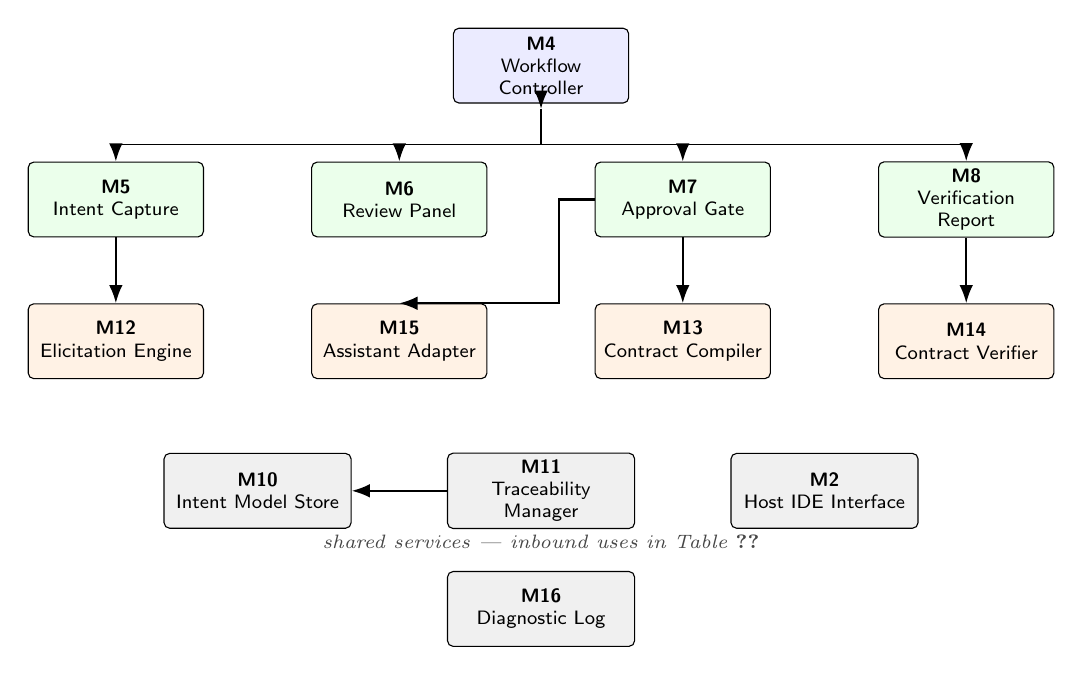
\begin{tikzpicture}[
  >=Latex,
  box/.style={
    draw, rounded corners=2pt, align=center,
    font=\scriptsize\sffamily, inner sep=2.5pt,
    minimum height=0.95cm, text width=2.05cm
  },
  arr/.style={->, thick},
  shared/.style={box, fill=gray!12, text width=2.2cm}
]
\node[box, fill=blue!8] (ctrl) at (0,0)
  {\textbf{M4}\\Workflow Controller};

\node[box, fill=green!8] (cap)  at (-5.4,-1.7)
  {\textbf{M5}\\Intent Capture};
\node[box, fill=green!8] (rev)  at (-1.8,-1.7)
  {\textbf{M6}\\Review Panel};
\node[box, fill=green!8] (gate) at (1.8,-1.7)
  {\textbf{M7}\\Approval Gate};
\node[box, fill=green!8] (rep)  at (5.4,-1.7)
  {\textbf{M8}\\Verification Report};

% Assist under Review column; Comp under Gate --- centres 3.6cm apart
\node[box, fill=orange!10] (elicit) at (-5.4,-3.5)
  {\textbf{M12}\\Elicitation Engine};
\node[box, fill=orange!10] (assist) at (-1.8,-3.5)
  {\textbf{M15}\\Assistant Adapter};
\node[box, fill=orange!10] (comp)   at (1.8,-3.5)
  {\textbf{M13}\\Contract Compiler};
\node[box, fill=orange!10] (ver)    at (5.4,-3.5)
  {\textbf{M14}\\Contract Verifier};

\node[shared] (store) at (-3.6,-5.4)
  {\textbf{M10}\\Intent Model Store};
\node[shared] (trace) at (0.0,-5.4)
  {\textbf{M11}\\Traceability Manager};
\node[shared] (host)  at (3.6,-5.4)
  {\textbf{M2}\\Host IDE Interface};
\node[shared] (log)   at (0.0,-6.9)
  {\textbf{M16}\\Diagnostic Log};

\node[font=\scriptsize\itshape, text=gray!55!black, align=center]
  at (0,-6.05)
  {shared services --- inbound uses in Table~\ref{TblUses}};

\coordinate (stem) at (0,-0.55);
\coordinate (bus) at (0,-1.0);
\draw[arr] (ctrl.south) -- (stem);
\draw (stem) -- (bus);
\draw (cap.north |- bus) -- (rep.north |- bus);
\draw[arr] (cap.north |- bus) -- (cap.north);
\draw[arr] (rev.north |- bus) -- (rev.north);
\draw[arr] (gate.north |- bus) -- (gate.north);
\draw[arr] (rep.north |- bus) -- (rep.north);

\draw[arr] (cap) -- (elicit);
% Gate->Comp vertical; Gate->Assist exits west so stems do not share a T-junction
\draw[arr] (gate) -- (comp);
\draw[arr] (gate.west) -- ++(-0.45,0) |- (assist.north);
\draw[arr] (rep) -- (ver);
\draw[arr] (trace) -- (store);
\end{tikzpicture}
\caption{Primary structural uses (arrow from $A$ to $B$ means $A$ uses $B$).
Module IDs match Section~\ref{SecMH}. Secondary uses of resources are listed in Table~\ref{TblUses}.}
\label{FigUH}
\end{figure}

\begin{table}[H]
\centering
\begin{tabular}{p{0.40\textwidth} p{0.50\textwidth}}
\toprule
\textbf{Module} & \textbf{Uses}\\
\midrule
M4 Workflow Controller & M5, M6, M7, M8, M2, M16\\
M5 Intent Capture & M12, M10, M2\\
M6 Review Panel & M2, M10\\
M7 Approval Gate & M10, M15, M13, M2, M16\\
M8 Verification Report & M14, M2\\
M12 Elicitation Engine & M10, M16\\
M13 Contract Compiler & M10, M11\\
M14 Contract Verifier & M10, M11, M16\\
M15 Coding Assistant Adapter & M10, M16\\
M11 Traceability Manager & M10\\
M10 Intent Model Store & ---\\
M2 Host IDE Interface & ---\\
M16 Diagnostic Log & ---\\
\bottomrule
\end{tabular}
\caption{Complete uses relation (matches MIS Uses subsections).}
\label{TblUses}
\end{table}

\section{User Interfaces}

Primary interaction is through host-IDE panels and commands provided by the
Host IDE Interface and Review Panel modules. Wireframe exploration of those
surfaces is the subject of the Fall Custom Document (Wireframe Report) and is
not duplicated here. The MG requires only that UI behaviour remain behind
\mref{mHost} and \mref{mReview} so that look-and-feel changes do not leak into
storage or verification modules.

\section{Design of Communication Protocols}

Communication with the AI coding assistant is confined to the Coding Assistant
Adapter module (\mref{mAssist}). The adapter hides encoding, transport, and
tool-registration decisions (\acref{acAssistant}). Behavioural modules depend
only on abstract services such as ``send approved implementation instruction''
or ``send revision request.'' No other module constructs assistant-channel
messages, which keeps coupling low and preserves replaceability of the
assistant (\acref{acAssistant}, MR3).

\section{Database Design}

\progname{} does not use a separate database server for the intent model. The
Intent Model Store (\mref{mStore}) persists structured artifacts in the project
workspace and versions them with Git (\uref{ucGitVersioning}). Schema, file
layout, and encoding of drafts versus approved artifacts are secrets of
\mref{mStore} (\acref{acSchema}); other modules obtain intent only through that
module's access programs.

\section{Timeline}

Work is tracked on the team GitHub project board and issues. For Design
Document Rev~-1:
\begin{itemize}
  \item Complete MG decomposition, uses relation, and traceability (this
    document).
  \item Complete MIS syntax for every leaf module.
  \item Align Wireframe Report insights with \mref{mReview} and \mref{mHost}.
\end{itemize}
Revision~0 will add MIS semantics, formal specification of at least one module,
and design reflection after peer module implementation.

\section{Generative AI Use Disclosure}

\subsection{AI Tools Used}

\begin{itemize}
  \item Cursor and Claude, used in the writing process for this Module Guide.
\end{itemize}

\subsection{How and Where Used}

\begin{itemize}
  \item \textbf{Completing sections from drafts.} Used to complete and fill
    out Module Guide sections based on the author's own drafts of anticipated
    changes, module hierarchy, secrets, and services.
  \item \textbf{Diagrams and tables.} Used to help produce and refine
    diagrams and tables, including the uses relation and traceability
    matrices.
  \item \textbf{Rubric review.} Used to evaluate the document against the
    Design Documentation rubric and to suggest areas of improvement, which
    the author then accepted, revised, or rejected.
\end{itemize}

\subsection{Verification of AI-Generated Content}

\begin{enumerate}
  \item Reviewed all AI-assisted expansions against the author's drafts before
    keeping them.
  \item Checked that secrets, uses relations, and traceability tables
    remain consistent with the SRS, Hazard Analysis, and companion MIS.
  \item Confirmed that low-level implementation detail was not introduced into
    secrets or services where the document should stay at the design-decision
    level.
\end{enumerate}

\newpage{}

\bibliographystyle{plainnat}
\bibliography{../../../refs/References}

\end{document}
